\chapter{oro-server, design \& use of a symbolic knowledge representation system for robotics}
\label{chapter|oroserver}

\fxnote{This chapter focuses on the \textbf{functional description} of
oro-server. It does not need to match the actual implementation.}

\section{Functional overview}
\label{sect|functional-overview}


We have adopted a centralized approach for knowledge management called
ORO~\cite{Lemaignan2010}. The platform is designed as a central
knowledge storage service implemented as a server where the robot
components can add or query statements at run-time. Figure~\ref{fig|oro-overview}
illustrates the main functional components of ORO.

\begin{figure}
\centering
  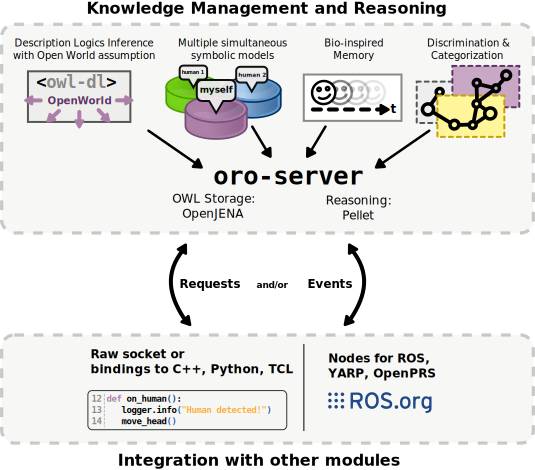
\includegraphics[width=0.8\linewidth]{oroserver/oro_architecture_functional.pdf}
  \caption{Overview of the ORO architecture.}
  \label{fig|oro-overview}
\end{figure}

At the core, ORO is build around the
OpenJena\footnote{\url{http://www.openjena.org}} ontology management library,
connected to the Pellet\footnote{\url{http://clarkparsia.com/pellet}}
reasoner.

A front-end accepts and manages connections to clients. The clients' requests
are processed by a set of internal modules: basic operations on statements,
but also higher cognitive and human-robot interaction related functionalities
are available. External plugins can also be easily added.

Besides acting as a facts database, the ORO platform exposes several
functions: operations on knowledge statements relying on inference (through a
continuous first-order logic classification process), management of
\emph{per-agent} symbolic models, and also higher cognitive and human-robot
interaction related functionalities like categorization of sets of concepts
or profiles of memory (that enable the robot to ``forget'' about some facts).

ORO also provides an event mechanism that allows components to be triggered
when specific events occur. A component can for instance subscribe to events
of kind \setstmt{?agent isVisible true, ?agent type Human}. As soon as the
perception layer detects a human in the robot's field of view and accordingly
updates the knowledge base, the executive layer is triggered. The event
framework also takes advantage of the inference capabilities of ORO. Thus an
event can be indirectly triggered if its triggering conditions can be
inferred to be true.


%%%%%%%%%%%%%%%%%%%%%%%%%%%%%%%%%%%%%%%%%%%%%%%%%%%%%%%%%%%%%%%%%%%%%%%%%%%%%%%
%%%%%%%%%%%%%%%%%%%%%%%%%%%%%%%%%%%%%%%%%%%%%%%%%%%%%%%%%%%%%%%%%%%%%%%%%%%%%%%
%%%%%%%%%%%%%%%%%%%%%%%%%%%%%%%%%%%%%%%%%%%%%%%%%%%%%%%%%%%%%%%%%%%%%%%%%%%%%%%

\section{The ORO Knowledge model}
\label{sect|knowledge-model}

\subsection{Expressiveness: What Can be Represented?}
\subsubsection{Open World and Close World Assumptions}
\subsubsection{Meta-cognition: knowledge on the knowledge}
Narrower, more technical dimension of the introspection.

%%%%%%%%%%
\subsection{How things are represented?}
\subsubsection{Role Representations}
Spatio-Temporal Representations:

\paragraph{Representation of time}
\paragraph{Representation of space}
\paragraph{Representation of events and actions}

\subsubsection{Context modeling}
\subsubsection{Possible-Worlds and representing what others know}

\paragraph{Multi-model representation for Persepective-taking}
\label{sect|alterite}

...

We present at section~\ref{sect|perspectivetaking}, page~\pageref{sect|perspectivetaking} an 3D real-time environment, SPARK, that allows to compute on-line several perspective aware symbolic properties.

\subsection{False beliefs and Theory Of Mind}
\label{sect|theory-of-mind}

\fxnote{Sally and Ann experiment}



\subsubsection{Introspection: Who am I? What can I do?}

%%%%%%%%%%
\subsection{Reasoning Techniques}

\subsubsection{Standard reasoning techniques}


Knowledge is stored as OWL/RDF ontologies in ORO. We use the Pellet reasoner to
classify them. This enables several type of reasoning:

\begin{itemize}
	\item reasoning on inheritance relations (\eg \emph{all bottles are containers}),
	\item property axioms
		\begin{itemize}
		\item entailments based on predicates' domain and range,
		\item cardinality constraints (including \concept{allValue}, 
		\concept{someValue}, \concept{hasValue}),
		\item property characteristics (symmetry, transitivity)
		\end{itemize}
	\item class restrictions like: \par \footnotesize \concept{Bottle} $\equiv$
		\concept{Artifact} {\bf that} (\concept{hasShape} {\bf value}
		\concept{cylinderShape})\footnote{This example uses the \emph{Manchester
		syntax}, \url{http://www.w3.org/TR/owl2-manchester-syntax/}} \normalsize
	\item set operations like: \par \footnotesize \concept{Color} $\equiv$ {\bf unionOf}(\concept{blue},
		\concept{green}, \concept{orange}, \concept{black}...) \normalsize
	\item generic SWRL ({\em Semantic Web Rule Language}) rules like: \par
		\footnotesize \concept{looksAt(?agt, ?obj)} $\land$
		\concept{pointsAt(?agt,?obj)} \par $\Rightarrow$ \concept{focusesOn(?agt, ?obj)}
		\normalsize 
	\end{itemize}

We provide in ORO accessors to query, add or remove all these properties and
restrictions (except the SWRL rules) at run-time. This allows knowledge
introspection and enables the robot to alter its own knowledge structures (the
so-called \emph{T-Box} model) during its life-time by adding new constraints
and properties to classes and predicates (we can for instance teach the robot
\emph{at runtime} that cats are animals, \ie \stmt{Cat rdfs:subClassOf
Animal}).


\paragraph{Decidability}

...


\subsubsection{Reasoning with uncertainty}
\subsubsection{(Non) Monotonic Reasoning}


\subsubsection{Memory}
\label{subssect|memory}


\subsubsection{Learning by modifying the knowledge structure}

%%%%%%%%%%%%%%%%%
\subsection{The left-overs: What ORO does not provide?}

\subsubsection{Representation of uncertainty and likelihood}

\subsubsection{Presupposition accommodation}
\subsubsection{Prediction, projection and diagnosis tasks}
\paragraph{Projection task}: determining whether or not some condition while
hold after a sequence of actions.

\paragraph{Legality task}: determining whether a sequence of action can be
performed starting in some initial state.

\paragraph{Diagnosis}: this corresponds to the ability to rewind on past events
in case of failure to provide possible explanation. This can be seen as the
temporal reverse of the projection task.


\subsubsection{Physics-based reasoning}
\subsubsection{Planning}
Making decision based on prediction




%%%%%%%%%%%%%%%%%%%%%%%%%%%%%%%%%%%%%%%%%%%%%%%%%%%%%%%%%%%%%%%%%%%%%%%%%%%%%%
%%%%%%%%%%%%%%%%%%%%%%%%%%%%%%%%%%%%%%%%%%%%%%%%%%%%%%%%%%%%%%%%%%%%%%%%%%%%%%
%%%%%%%%%%%%%%%%%%%%%%%%%%%%%%%%%%%%%%%%%%%%%%%%%%%%%%%%%%%%%%%%%%%%%%%%%%%%%%

\section{Knowledge instanciation: the OpenRobots Common-Sense Ontology}

How much knowledge is available? Which content? How big is the knowledge base?

\subsection{Designing the \textsc{OpenRobots} common-sense ontology}
\label{sect|commonsense-design}


%%%%%%%%%%%%%%%%%%%%%%%%%%%%%%%%%%%%%%%%%%%%%%%%%%%%%%%%%%%%%%%%%%%%%%%%%%%%%%
%%%%%%%%%%%%%%%%%%%%%%%%%%%%%%%%%%%%%%%%%%%%%%%%%%%%%%%%%%%%%%%%%%%%%%%%%%%%%%
%%%%%%%%%%%%%%%%%%%%%%%%%%%%%%%%%%%%%%%%%%%%%%%%%%%%%%%%%%%%%%%%%%%%%%%%%%%%%%
\subsection{Presupposition accomodation}
\label{sect|presupposition-accomodation}

\fxerror{TDB: this should show that the system can be enriched with facts that
are not perceived, but teached to the robot. How to demonstrate that?}

